\documentclass[11pt]{article}

\usepackage{fontspec}
\usepackage{graphicx}
\usepackage{amsmath}
\usepackage{booktabs}
\usepackage{float}
\usepackage{array}
\usepackage{hyperref}
\usepackage[a4paper, left=2cm, right=2cm, top=2cm, bottom=2.5cm]{geometry}

\setmainfont{texgyretermes}[
    Extension=.otf,
    UprightFont=*-regular,
    BoldFont=*-bold,
    ItalicFont=*-italic,
    BoldItalicFont=*-bolditalic
]

\title{DD2356 VT26 Project Report\\Pengyu Wang's Part: MPI Scaling and GPU Offloading}
\author{Group 26}
\date{}

\begin{document}
\maketitle

\section{Design and Implementation}
\label{sec:wang-design}

\subsection{MPI Decomposition and Communication}
\label{subsec:wang-mpi}

The MPI implementation uses a destination-node block decomposition. For a graph
with $N$ vertices and $P$ MPI ranks, rank $r$ owns a contiguous vertex interval
$[start_r,end_r)$ and computes only the corresponding entries of the next
PageRank vector. The graph is stored in the same incoming-edge CSR layout as the
serial baseline: \texttt{row\_ptr[v]} to \texttt{row\_ptr[v+1]-1} enumerates
all source vertices contributing to destination vertex $v$. To keep the first
distributed-memory version simple and easy to verify, each rank stores the full
CSR graph and the full current PageRank vector, while only the newly computed
block \texttt{pr\_new[start:end]} is rank-local.

The graph is loaded on rank 0 and distributed to the other ranks with
\texttt{MPI\_Bcast}. Each PageRank iteration then performs the following
communication:
\begin{enumerate}
    \item One scalar \texttt{MPI\_Allreduce} for the global dangling-node mass.
    \item One scalar \texttt{MPI\_Allreduce} for the global $L_1$ convergence
          difference.
    \item One \texttt{MPI\_Allgatherv} to assemble the full next PageRank vector
          on every rank.
\end{enumerate}
The per-iteration cost can therefore be modeled as
\[
T_{\mathrm{iter}}(P) \approx T_{\mathrm{comp}}\left(\frac{M}{P}\right)
    + 2T_{\mathrm{allreduce}}(P)
    + T_{\mathrm{allgatherv}}(N,P),
\]
where $M$ is the number of edges. This model predicts that the implementation
will be communication-bound for small graphs or when the full-vector
\texttt{Allgatherv} dominates the reduced local sparse update.

\subsection{Hybrid MPI+OpenMP}
\label{subsec:wang-hybrid}

The hybrid version keeps the same MPI node-block decomposition and adds OpenMP
parallelism inside each MPI rank. The dangling-node mass and convergence checks
use OpenMP reductions, while the sparse incoming-edge PageRank update uses
\texttt{\#pragma omp parallel for schedule(dynamic, 256)}. The dynamic schedule
was chosen because real graphs such as \texttt{polblogs.csv} have highly
irregular in-degree distributions; assigning a fixed number of destination
vertices to each thread can leave some threads with many more incoming edges
than others.

For comparison with the GPU-offloading path, the group hybrid implementation
supports fixed-core experiments with configurations
\texttt{1x16}, \texttt{2x8}, \texttt{4x4}, \texttt{8x2}, and \texttt{16x1},
where the first number is the MPI rank count $P$ and the second number is the
OpenMP thread count $N$ per rank. These runs are intended to identify whether
the best performance comes from fewer MPI ranks with more threads, or more MPI
ranks with less intra-rank threading.

\subsection{OpenMP GPU Offloading}
\label{subsec:wang-gpu}

The GPU comparison path is implemented with OpenMP target offloading and has
two variants. The \texttt{naive} baseline remaps graph and PageRank data for
target kernels, while the \texttt{persistent} version establishes an outer
device-data region, retains the CSR arrays and ping-pong PageRank buffers on
the device across all iterations, and performs dangling-mass and convergence
reductions on the target. Formal runs set \path{PR_REQUIRE_DEVICE=1}, so
CPU fallback causes a failed run rather than an accepted measurement. Since
the course allocation did not provide a Dardel GPU job, the confirmed-device
measurement used the DD2356 Small GPU server: an NVIDIA H100
\texttt{MIG 1g.10gb} allocation. A Hybrid \texttt{4x2} control was run on
the CPU resources of that same server.

\section{Correctness Evaluation}
\label{sec:wang-correctness}

All parallel outputs were compared against the serial PageRank reference using
the repository verifier and a tolerance of $10^{-6}$. The MPI implementation
passed the full nine-dataset correctness suite on Dardel for $P=1,2,4$ ranks,
and the formal Dardel scaling experiments passed for all measured
$P=1,2,4,8,16$ cases in a two-node \texttt{main}-partition job. On the school cluster, the MPI strong-scaling runs for both
\texttt{polblogs.csv} and \texttt{synthetic\_100k\_1m.csv}, as well as the
weak-scaling sequence up to the 200k-node/2M-edge graph, passed for all
measured rank counts. The hybrid fixed-core runs passed for every tested
$(P,N)$ combination on both datasets. The maximum errors are at machine
precision scale, e.g. at most $1.04\times 10^{-17}$ in the Dardel
\texttt{polblogs.csv} MPI run. The formal GPU run additionally passed all nine
course datasets with \texttt{executed\_on\_device=YES}; both timed GPU
variants passed on the synthetic comparison graph with maximum error
$1.02\times 10^{-20}$.

\begin{table}[H]
\centering
\caption{Correctness summary for Wang-owned implementations.}
\label{tab:wang-correctness}
\small
\begin{tabular}{p{0.20\textwidth}p{0.22\textwidth}p{0.28\textwidth}p{0.20\textwidth}}
\toprule
Implementation & Dataset scope & Configuration & Result \\
\midrule
MPI & 9 course datasets & 1, 2, 4 ranks on Dardel & PASS, tol. $10^{-6}$ \\
MPI & Dardel scaling datasets & 1--16 ranks, two \texttt{main} nodes & PASS, tol. $10^{-6}$ \\
MPI & 2 cluster datasets & 1, 2, 4, 8, 16 ranks on school cluster & PASS, tol. $10^{-6}$ \\
MPI & cluster weak-scaling sequence & 1 to 16 ranks; up to 200k nodes / 2M edges & PASS, tol. $10^{-6}$ \\
Hybrid MPI+OpenMP & 2 cluster datasets & fixed 16 cores: \texttt{1x16} to \texttt{16x1} & PASS, tol. $10^{-6}$ \\
OpenMP target GPU & 9 course datasets & H100 MIG persistent target path; device verified & PASS vs. serial \\
\bottomrule
\end{tabular}
\end{table}

\section{Scaling Evaluation}
\label{sec:wang-scaling}

\subsection{Dardel MPI Strong Scaling}
\label{subsec:wang-dardel-strong}

The formal Dardel run was submitted as Slurm job \texttt{20957663} on the
\texttt{main} partition using compute nodes \texttt{nid001120} and
\texttt{nid001121}. A placement probe outside each measured interval records
that every $P=2,4,8,16$ case is balanced across both nodes; the $P=1$ row is
the one-node reference. Table~\ref{tab:wang-polblogs-strong} reports the
strong-scaling result for the course \texttt{polblogs.csv} graph. The graph is small
($1224$ vertices and $19090$ edges), so the communication overhead is much
larger than the useful local sparse update once more than one rank is used.

\begin{table}[H]
\centering
\caption{Two-node MPI strong scaling on Dardel for \texttt{polblogs.csv} (directed).}
\label{tab:wang-polblogs-strong}
\begin{tabular}{rrrrrrr}
\toprule
Ranks & Runs & PR time (s) & Comm frac. & Speedup & Efficiency & Imbalance \\
\midrule
1  & 5 & 0.002364 & 0.0463 & 1.000000 & 1.000000 & 1.000 \\
2  & 5 & 0.003274 & 0.9144 & 0.722008 & 0.361004 & 1.887 \\
4  & 5 & 0.003406 & 0.9637 & 0.694110 & 0.173528 & 3.129 \\
8  & 5 & 0.003346 & 0.9805 & 0.706557 & 0.088320 & 4.412 \\
16 & 5 & 0.003732 & 0.9896 & 0.633474 & 0.039592 & 4.536 \\
\bottomrule
\end{tabular}
\end{table}

To separate graph-size effects from implementation effects, the same experiment
was repeated on a larger synthetic graph with $100000$ vertices and
$1000000$ edges. The larger graph has much better block balance
(max/average in-edge imbalance around $1.05$). Table~\ref{tab:wang-synth-strong}
shows useful scaling through $P=8$, where speedup reaches $2.98\times$, but
the speedup declines at $P=16$ as collective communication grows.

\begin{table}[H]
\centering
\caption{Two-node MPI strong scaling on Dardel for \texttt{synthetic\_100k\_1m.csv} (directed).}
\label{tab:wang-synth-strong}
\begin{tabular}{rrrrrrr}
\toprule
Ranks & Runs & PR time (s) & Comm frac. & Speedup & Efficiency & Imbalance \\
\midrule
1  & 5 & 0.036330 & 0.0395 & 1.000000 & 1.000000 & 1.000 \\
2  & 5 & 0.020386 & 0.1462 & 1.782080 & 0.891040 & 1.035 \\
4  & 5 & 0.012707 & 0.3017 & 2.859025 & 0.714756 & 1.044 \\
8  & 5 & 0.012205 & 0.5257 & 2.976714 & 0.372089 & 1.047 \\
16 & 5 & 0.014107 & 0.7600 & 2.575258 & 0.160954 & 1.051 \\
\bottomrule
\end{tabular}
\end{table}

For the synthetic graph, communication fraction increases from $0.1462$ at
$P=2$ to $0.7600$ at $P=16$. The work imbalance remains only $1.051$ at
$P=16$, whereas \texttt{MPI\_Allgatherv} alone grows to an average of
$0.008713$ s. Thus the two-node result demonstrates useful parallelism for a
larger graph, but also shows that replicated-vector collectives limit
high-rank efficiency.

\begin{figure}[H]
\centering
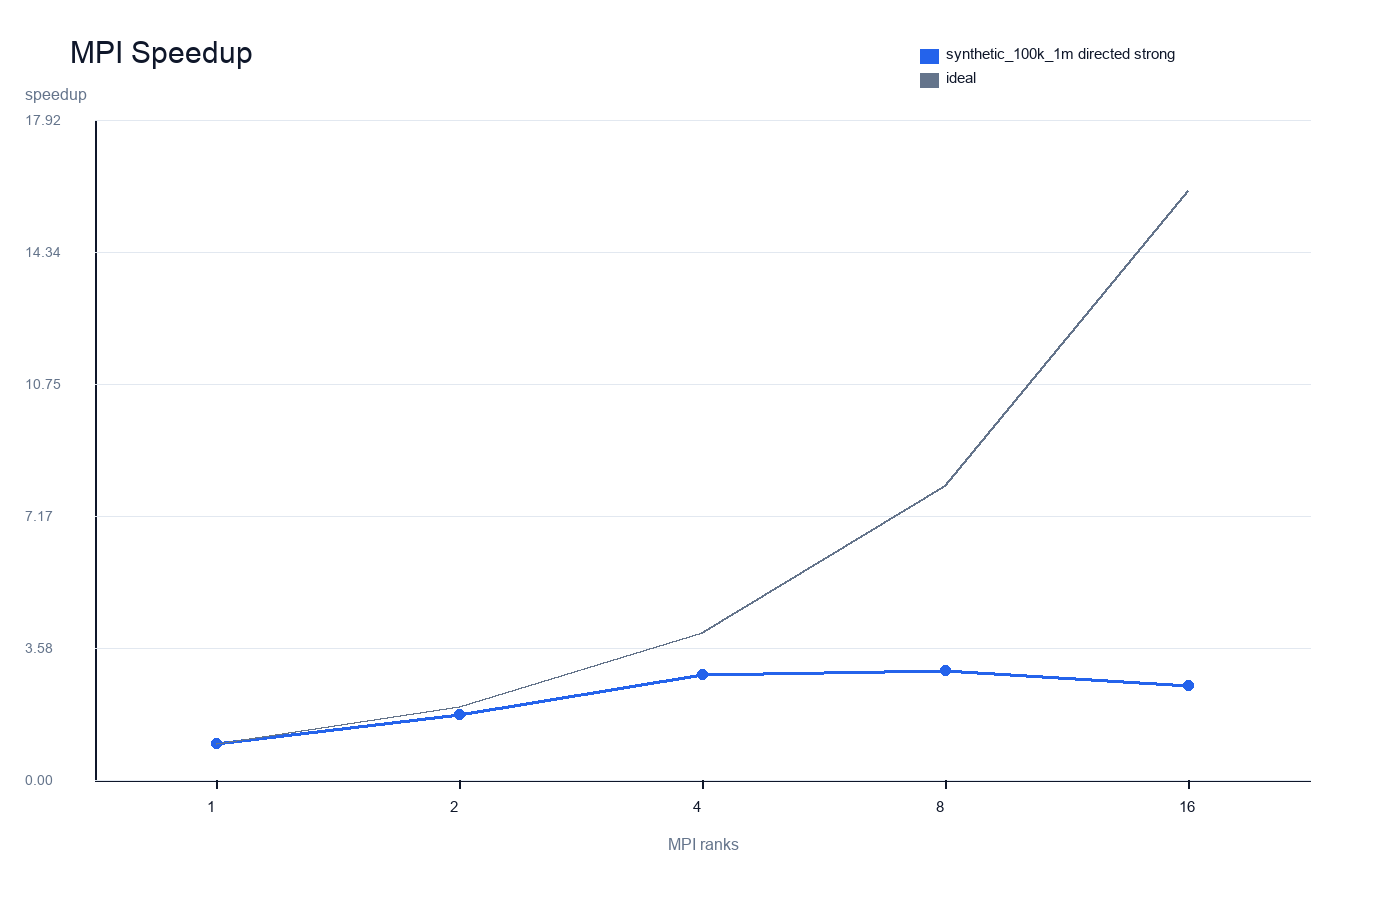
\includegraphics[width=0.48\textwidth]{results/figures/dardel_multinode_strong/mpi_speedup.png}
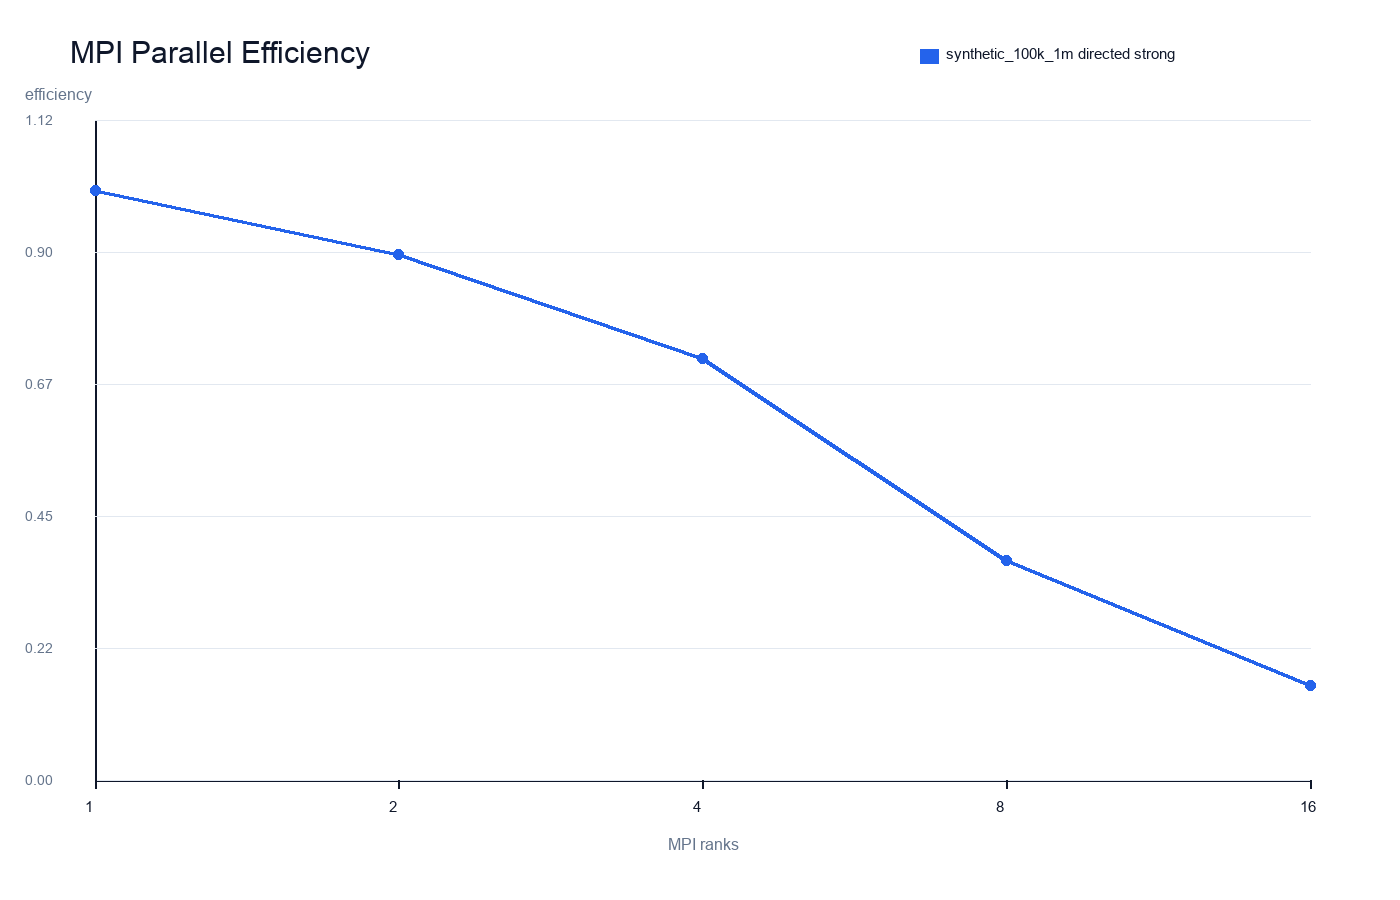
\includegraphics[width=0.48\textwidth]{results/figures/dardel_multinode_strong/mpi_efficiency.png}
\caption{Dardel two-node MPI speedup and parallel efficiency for the synthetic graph.}
\label{fig:wang-mpi-speedup-efficiency}
\end{figure}

\begin{figure}[H]
\centering
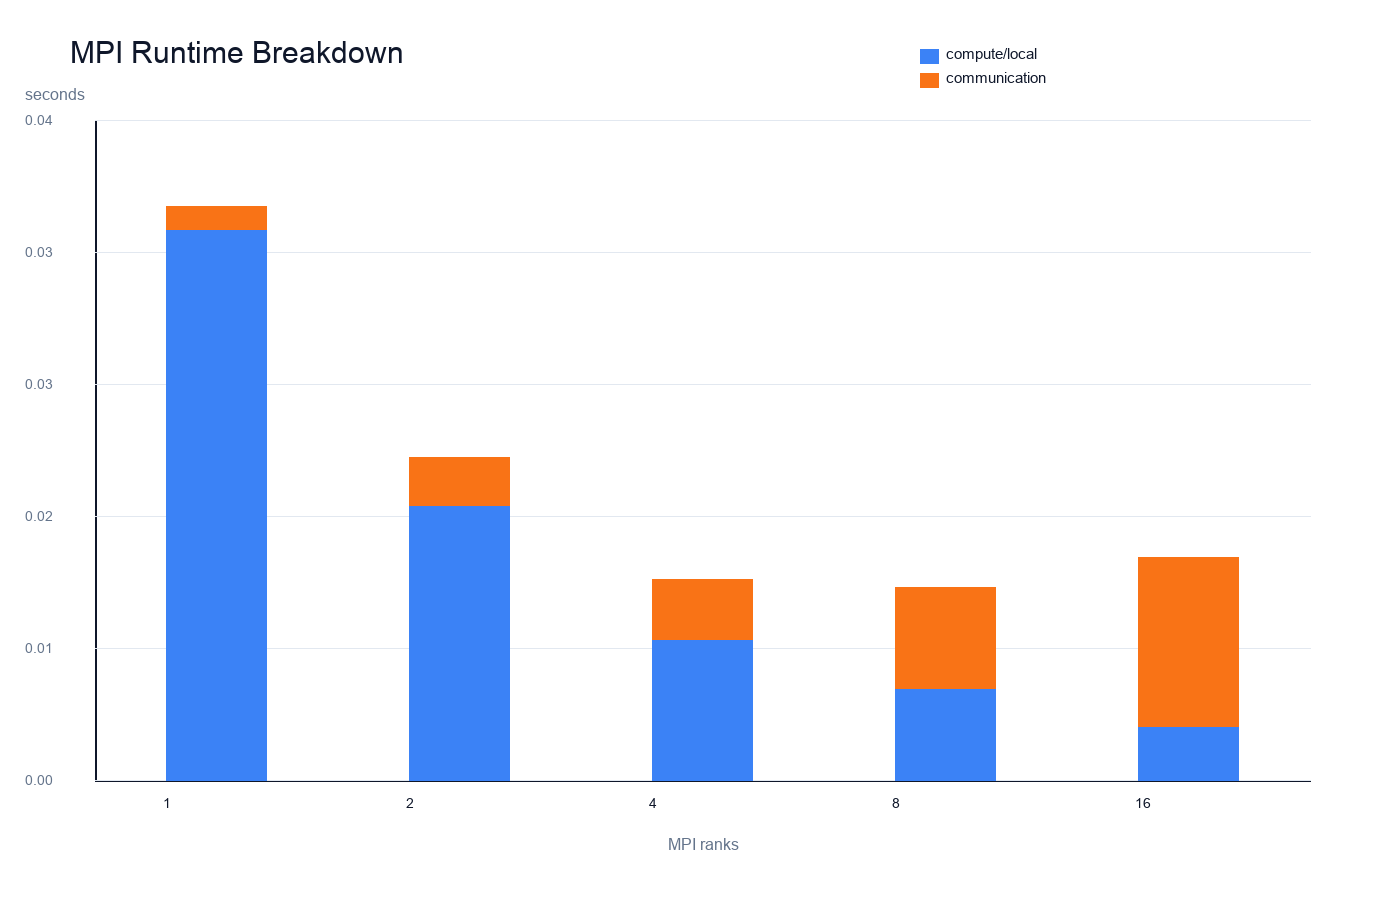
\includegraphics[width=0.48\textwidth]{results/figures/dardel_multinode_strong/mpi_runtime_breakdown.png}
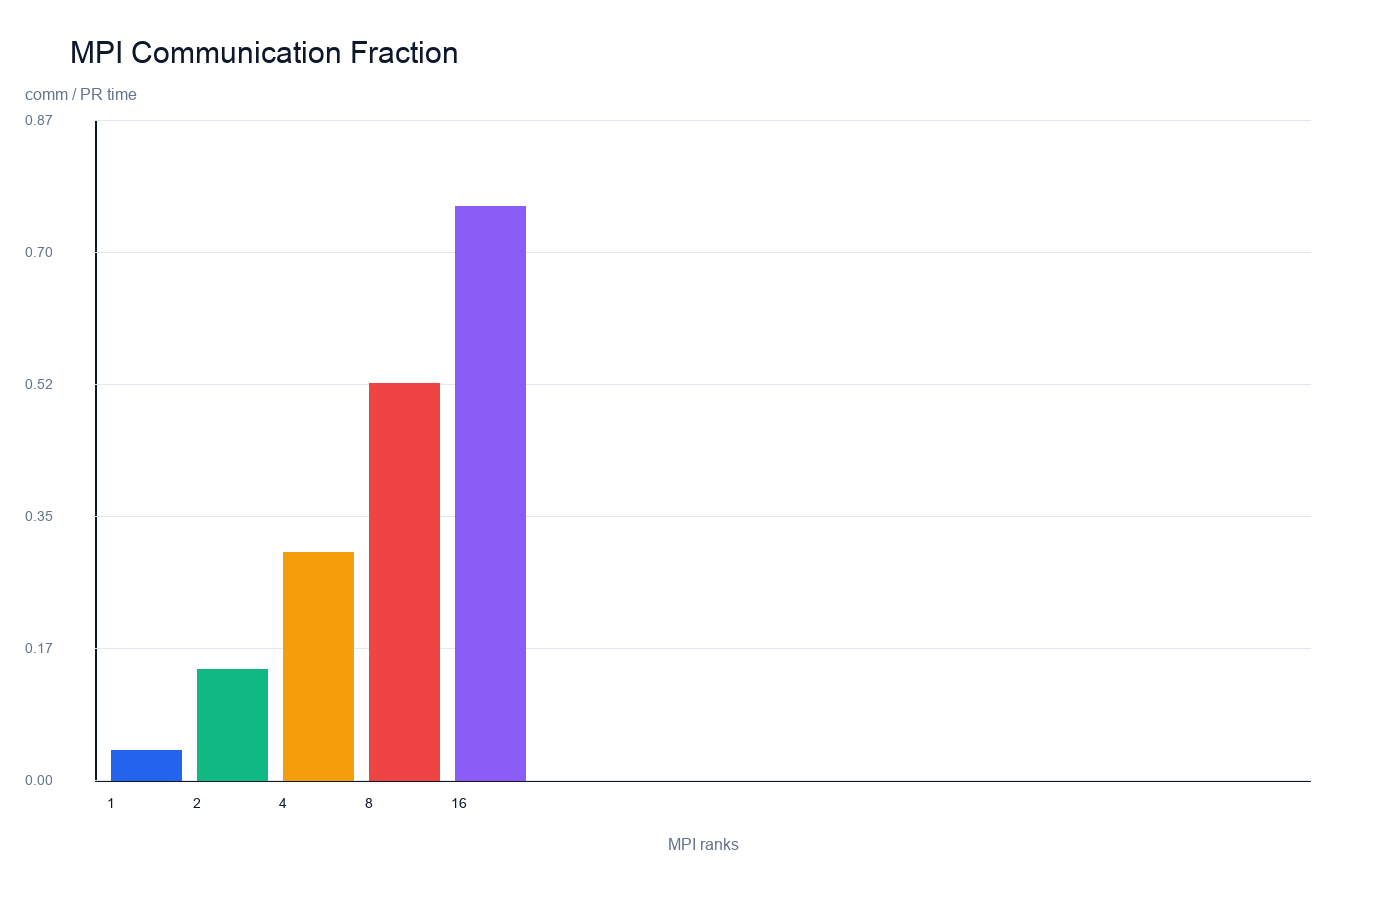
\includegraphics[width=0.48\textwidth]{results/figures/dardel_multinode_strong/mpi_comm_fraction.png}
\caption{Dardel two-node MPI runtime breakdown and communication fraction.}
\label{fig:wang-mpi-runtime-comm}
\end{figure}

\begin{figure}[H]
\centering
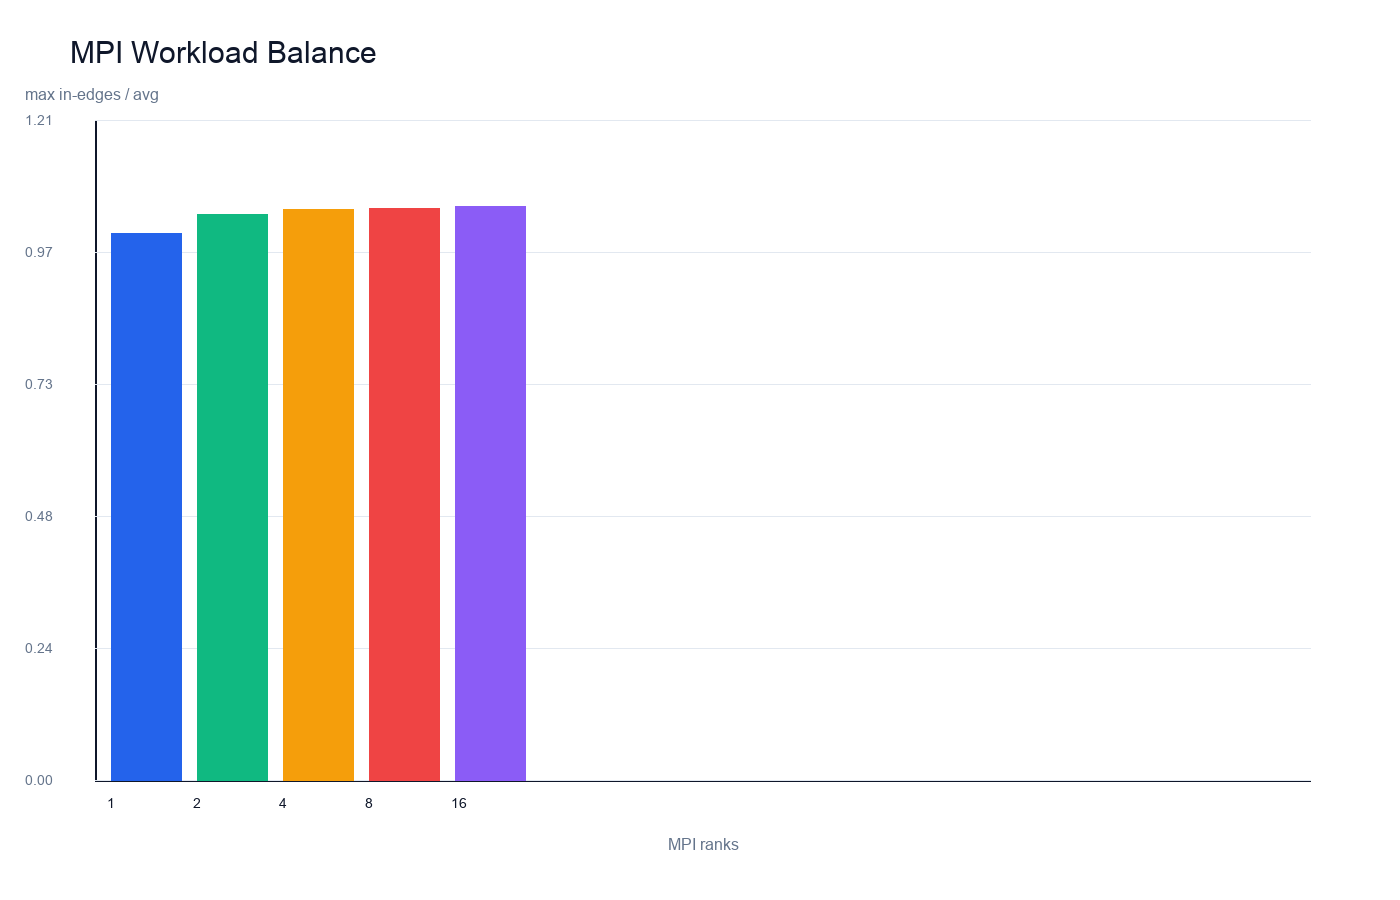
\includegraphics[width=0.55\textwidth]{results/figures/dardel_multinode_strong/mpi_workload_balance.png}
\caption{Dardel two-node MPI workload imbalance measured as max in-edges divided by average in-edges.}
\label{fig:wang-mpi-workload}
\end{figure}

\subsection{Dardel MPI Weak Scaling}
\label{subsec:wang-dardel-weak}

Weak scaling keeps the per-rank graph size approximately fixed while increasing
the number of ranks. For this project I used $12500$ vertices and $125000$
edges per rank, so the required 16-rank experiment uses a
$200000$-vertex, $2000000$-edge synthetic graph. This is a different
experiment from strong scaling: strong scaling fixes the graph size, while weak
scaling grows the global graph so each rank receives similar local work.
The same two-node placement policy as in strong scaling is used for all
multi-rank rows.

\begin{table}[H]
\centering
\caption{Two-node MPI weak scaling on Dardel with 125k edges per rank.}
\label{tab:wang-dardel-weak}
\scriptsize
\begin{tabular}{lrrrrrrr}
\toprule
Dataset & Ranks & Nodes & Edges & PR time (s) & Comm frac. & Weak eff. & Status \\
\midrule
\texttt{weak\_1rank\_12500\_125000}    & 1  & 12500  & 125000  & 0.003778 & 0.0353 & 1.000000000 & PASS \\
\texttt{weak\_2rank\_25000\_250000}    & 2  & 25000  & 250000  & 0.005837 & 0.3138 & 0.647216036 & PASS \\
\texttt{weak\_4rank\_50000\_500000}    & 4  & 50000  & 500000  & 0.006134 & 0.3398 & 0.615898790 & PASS \\
\texttt{weak\_8rank\_100000\_1000000}  & 8  & 100000 & 1000000 & 0.011932 & 0.5365 & 0.316600181 & PASS \\
\texttt{weak\_16rank\_200000\_2000000} & 16 & 200000 & 2000000 & 0.044137 & 0.5960 & 0.085592587 & PASS \\
\bottomrule
\end{tabular}
\end{table}

The 16-rank row satisfies the required weak-scaling case and confirms that the
dynamic graph reader can process the larger 200k-node input. However, weak
efficiency drops sharply because the replicated-vector algorithm still
communicates the full global PageRank vector every iteration. In the 16-rank
weak-scaling run, \texttt{MPI\_Allgatherv} alone averages $0.020449$ s out of
$0.044137$ s PageRank time, so increasing local work per rank is not enough to
hide the global communication cost.

\begin{figure}[H]
\centering
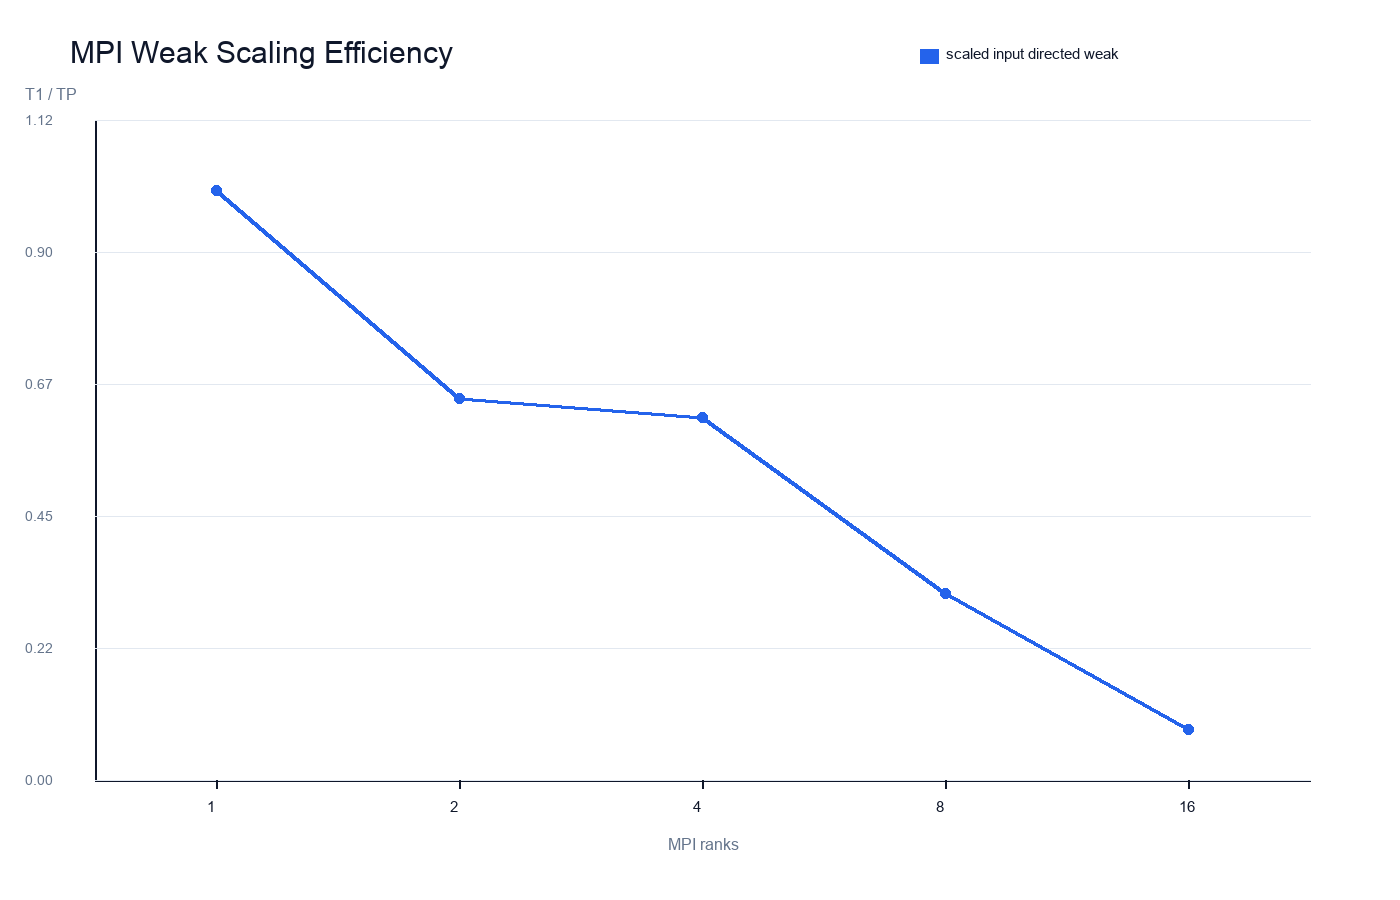
\includegraphics[width=0.48\textwidth]{results/figures/dardel_multinode_weak/mpi_weak_efficiency.png}
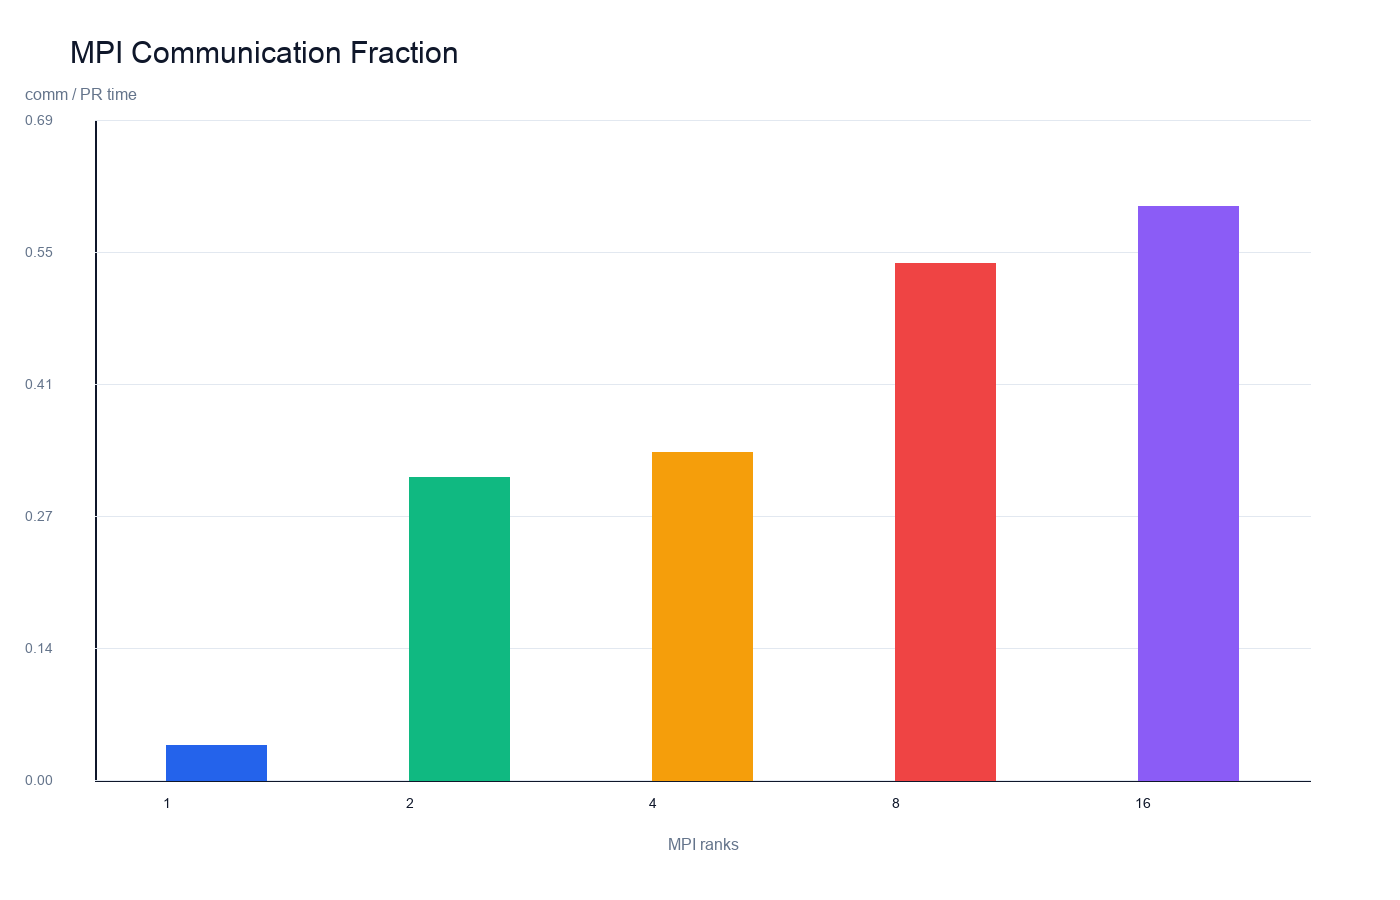
\includegraphics[width=0.48\textwidth]{results/figures/dardel_multinode_weak/mpi_comm_fraction.png}
\caption{Dardel two-node weak-scaling efficiency and communication fraction.}
\label{fig:wang-dardel-weak}
\end{figure}

\subsection{School-Cluster MPI Strong Scaling}
\label{subsec:wang-school-strong}

The same MPI profiler was run on the school cluster. Table~\ref{tab:wang-cluster-polblogs}
shows that the small \texttt{polblogs.csv} graph remains communication-bound:
the one-rank average PR time is only $0.001484$ s, and adding ranks increases
the communication fraction to $0.84$--$0.99$. This is the expected regime where
collective synchronization dominates useful work.

\begin{table}[H]
\centering
\caption{MPI strong scaling on the school cluster for \texttt{polblogs.csv} (directed).}
\label{tab:wang-cluster-polblogs}
\begin{tabular}{rrrrrrr}
\toprule
Ranks & Runs & PR time (s) & Comm frac. & Speedup & Efficiency & Imbalance \\
\midrule
1  & 5 & 0.001484 & 0.0142 & 1.000000 & 1.000000 & 1.000 \\
2  & 5 & 0.001889 & 0.8397 & 0.785472 & 0.392736 & 1.887 \\
4  & 5 & 0.002927 & 0.8878 & 0.506936 & 0.126734 & 3.129 \\
8  & 5 & 0.002461 & 0.9801 & 0.602844 & 0.075356 & 4.412 \\
16 & 5 & 0.002844 & 0.9898 & 0.521733 & 0.032608 & 4.536 \\
\bottomrule
\end{tabular}
\end{table}

For the larger synthetic graph, the school-cluster MPI run scales up to four
ranks before communication dominates. Table~\ref{tab:wang-cluster-synth} shows
the best average speedup at $P=4$ with $2.14\times$ speedup and $0.534$
parallel efficiency. From $P=8$ onward, the communication fraction rises from
$0.44$ to $0.75$ and then $0.85$, so the extra ranks no longer compensate for
the collective communication cost. The raw rank-16 measurements include one
large outlier (\texttt{PR time = 0.070486 s}); therefore the table keeps the
summary average as the main metric while the median rank-16 time
($0.012609$ s) is useful as a robustness check.

\begin{table}[H]
\centering
\caption{MPI strong scaling on the school cluster for \texttt{synthetic\_100k\_1m.csv} (directed).}
\label{tab:wang-cluster-synth}
\begin{tabular}{rrrrrrr}
\toprule
Ranks & Runs & PR time (s) & Comm frac. & Speedup & Efficiency & Imbalance \\
\midrule
1  & 5 & 0.027228 & 0.0137 & 1.000000 & 1.000000 & 1.000 \\
2  & 5 & 0.017646 & 0.1766 & 1.543006 & 0.771503 & 1.035 \\
4  & 5 & 0.012738 & 0.4356 & 2.137590 & 0.534398 & 1.044 \\
8  & 5 & 0.015967 & 0.7505 & 1.705301 & 0.213163 & 1.047 \\
16 & 5 & 0.023347 & 0.8478 & 1.166240 & 0.072890 & 1.051 \\
\bottomrule
\end{tabular}
\end{table}

\begin{figure}[H]
\centering
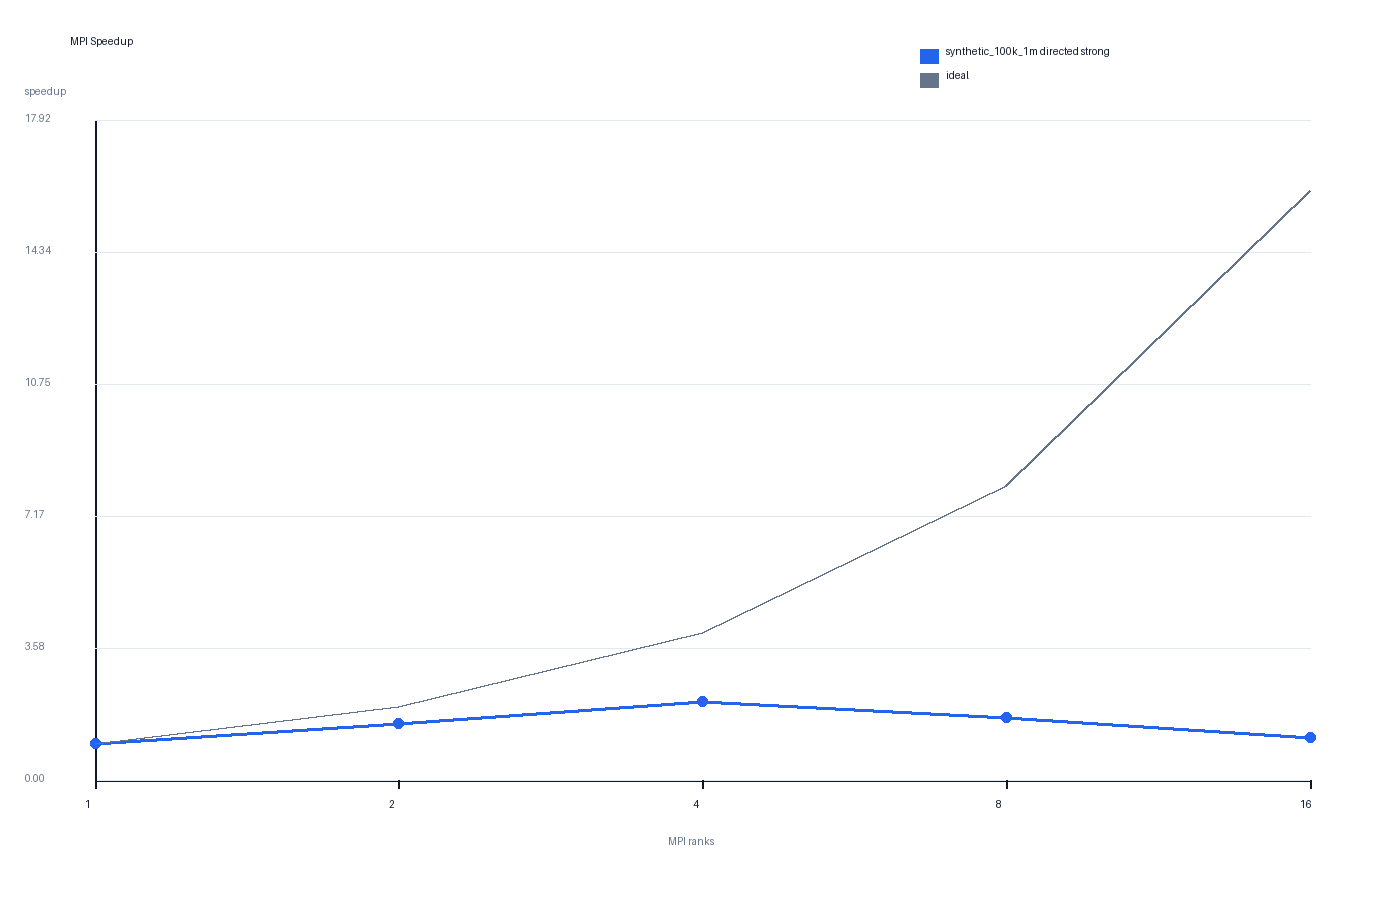
\includegraphics[width=0.48\textwidth]{results/figures/mpi_speedup_cluster.png}
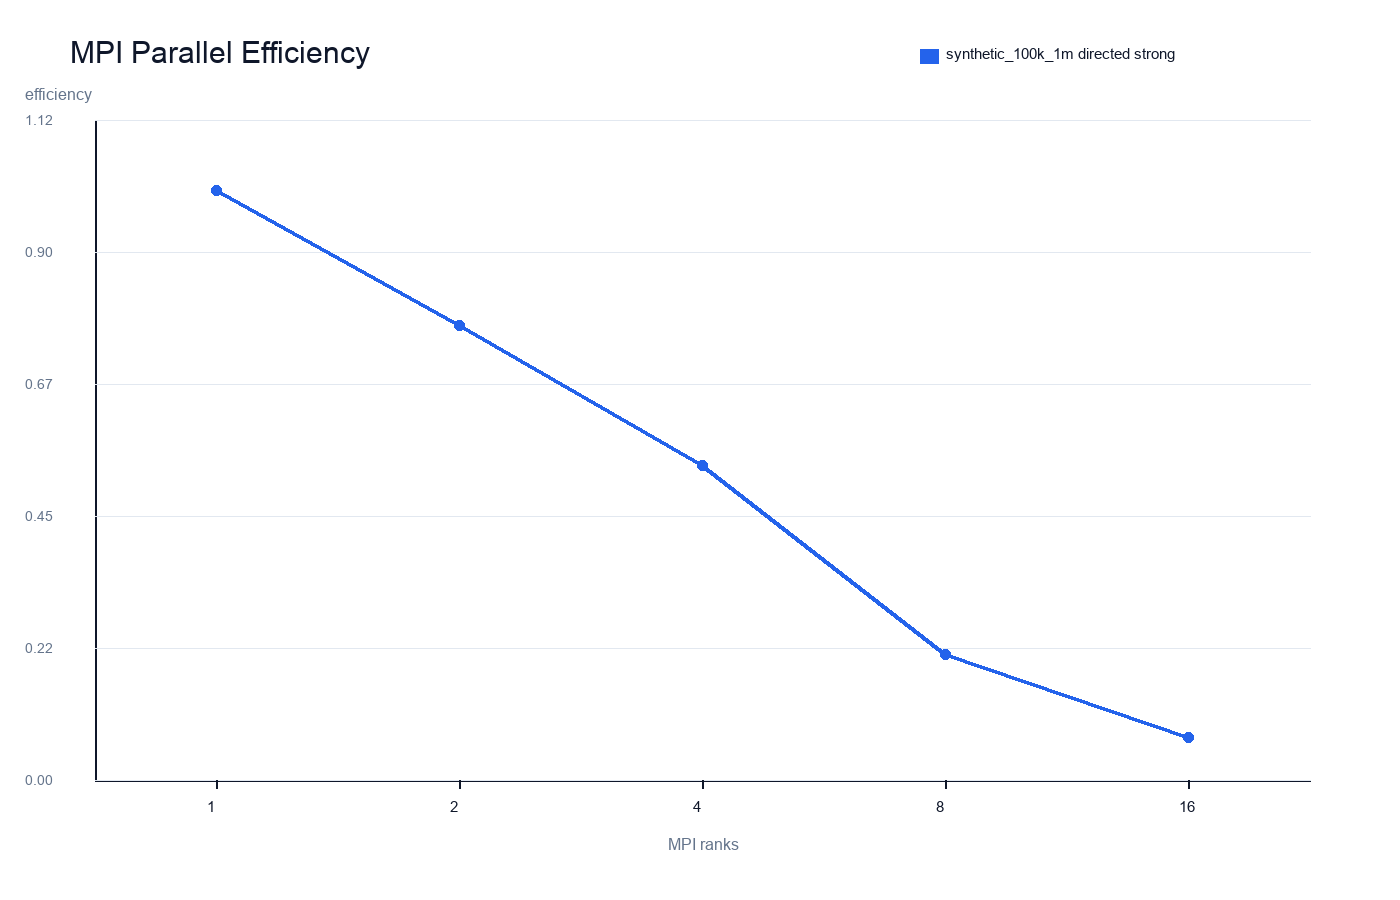
\includegraphics[width=0.48\textwidth]{results/figures/mpi_efficiency_cluster.png}
\caption{School-cluster MPI speedup and parallel efficiency for \texttt{synthetic\_100k\_1m.csv}.}
\label{fig:wang-cluster-speedup-efficiency}
\end{figure}

\begin{figure}[H]
\centering
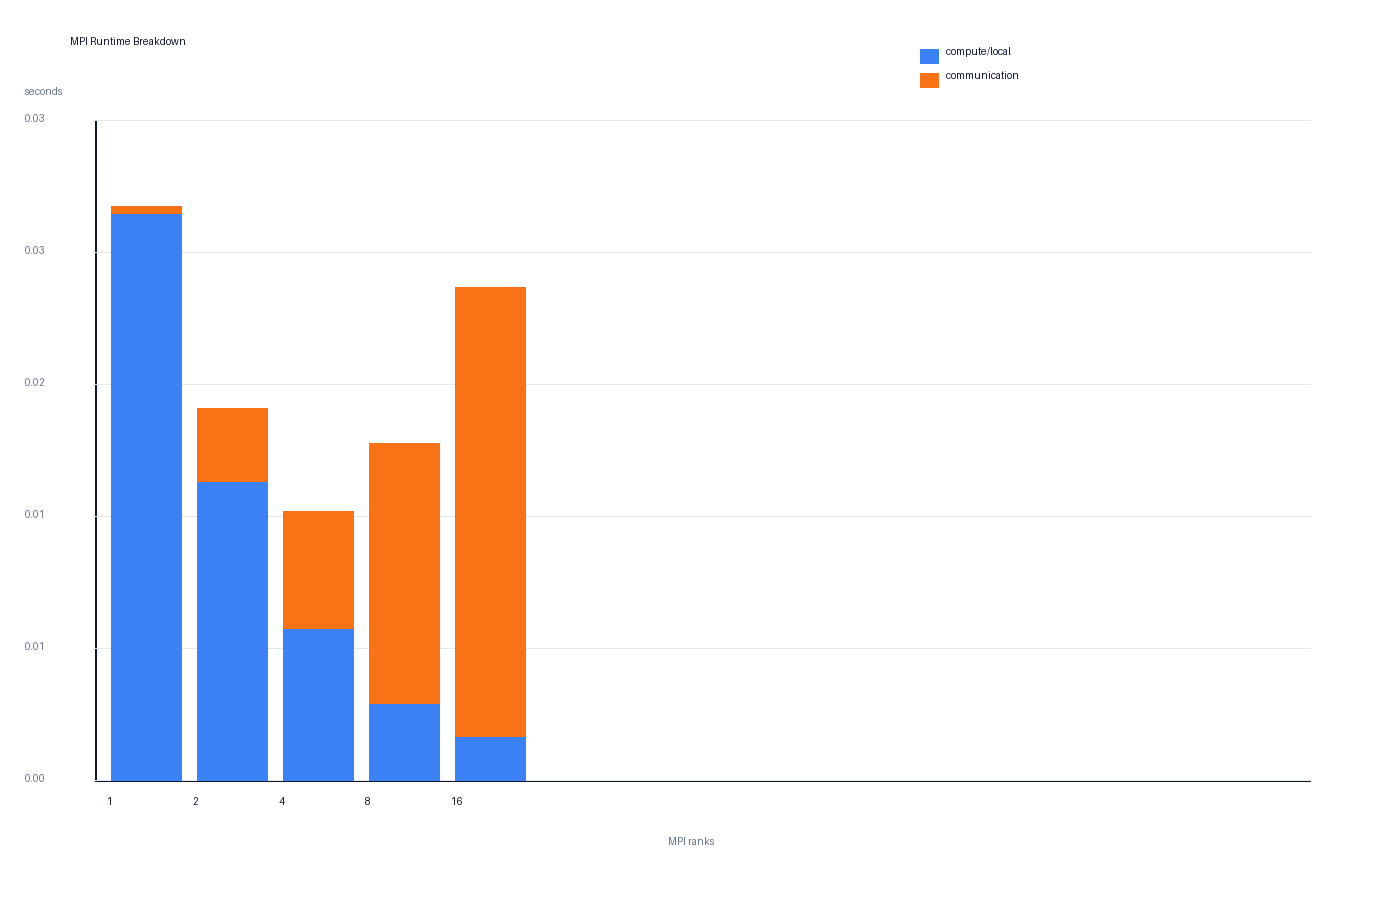
\includegraphics[width=0.48\textwidth]{results/figures/mpi_runtime_breakdown_cluster.png}
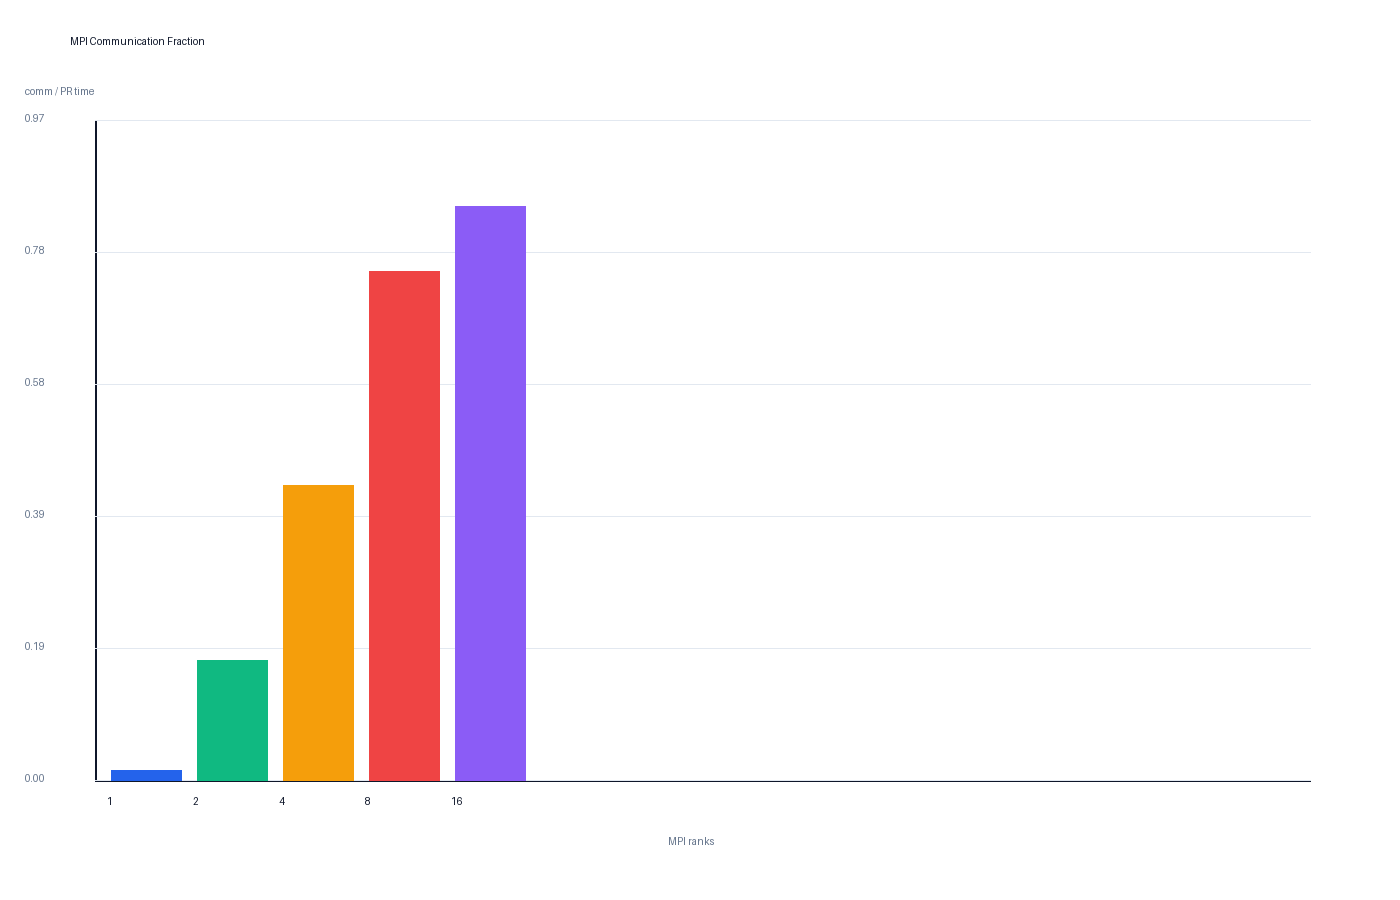
\includegraphics[width=0.48\textwidth]{results/figures/mpi_comm_fraction_cluster.png}
\caption{School-cluster MPI runtime breakdown and communication fraction.}
\label{fig:wang-cluster-runtime-comm}
\end{figure}

\begin{figure}[H]
\centering
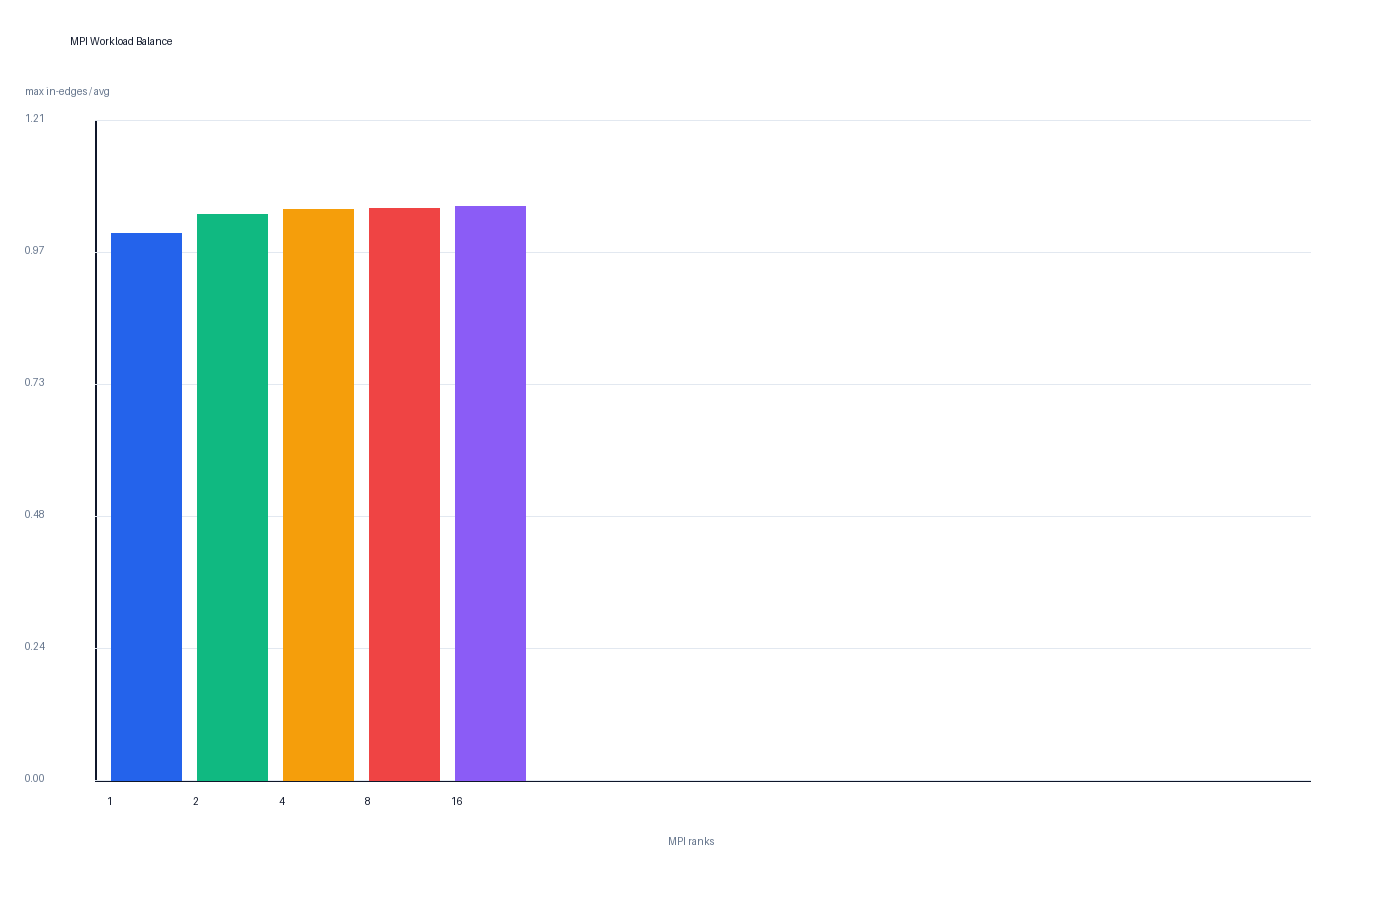
\includegraphics[width=0.55\textwidth]{results/figures/mpi_workload_balance_cluster.png}
\caption{School-cluster MPI workload imbalance for \texttt{synthetic\_100k\_1m.csv}.}
\label{fig:wang-cluster-workload}
\end{figure}

\subsection{School-Cluster MPI Weak Scaling}
\label{subsec:wang-school-weak}

The school-cluster weak-scaling experiment used the same generated graph
instances as the Dardel experiment, with $125000$ edges assigned per rank and
a 16-rank maximum input of $200000$ vertices and $2000000$ edges. Equality of
the per-rank in-edge distributions in the two result CSV files confirms that
the comparisons are made on identical graph instances.

\begin{table}[H]
\centering
\caption{MPI weak scaling on the school cluster with 125k edges per rank.}
\label{tab:wang-cluster-weak}
\scriptsize
\begin{tabular}{lrrrrrrr}
\toprule
Dataset & Ranks & Nodes & Edges & PR time (s) & Comm frac. & Weak eff. & Status \\
\midrule
\texttt{weak\_1rank\_12500\_125000}    & 1  & 12500  & 125000  & 0.003310 & 0.0123 & 1.000000000 & PASS \\
\texttt{weak\_2rank\_25000\_250000}    & 2  & 25000  & 250000  & 0.005345 & 0.2442 & 0.619298836 & PASS \\
\texttt{weak\_4rank\_50000\_500000}    & 4  & 50000  & 500000  & 0.007542 & 0.4821 & 0.438951947 & PASS \\
\texttt{weak\_8rank\_100000\_1000000}  & 8  & 100000 & 1000000 & 0.011587 & 0.5887 & 0.285694560 & PASS \\
\texttt{weak\_16rank\_200000\_2000000} & 16 & 200000 & 2000000 & 0.024371 & 0.6814 & 0.135833573 & PASS \\
\bottomrule
\end{tabular}
\end{table}

Although the school cluster performs substantially better than the measured
Dardel job, its weak efficiency still falls from $1.0$ to $0.1358$ by 16
ranks. The per-rank incoming-edge imbalance remains small (at most $1.051$),
while communication consumes $68.14\%$ of PageRank time at 16 ranks.
Therefore, the weak-scaling deterioration is attributable primarily to the
replicated-vector collectives, rather than to uneven sparse work assignment.

\begin{figure}[H]
\centering
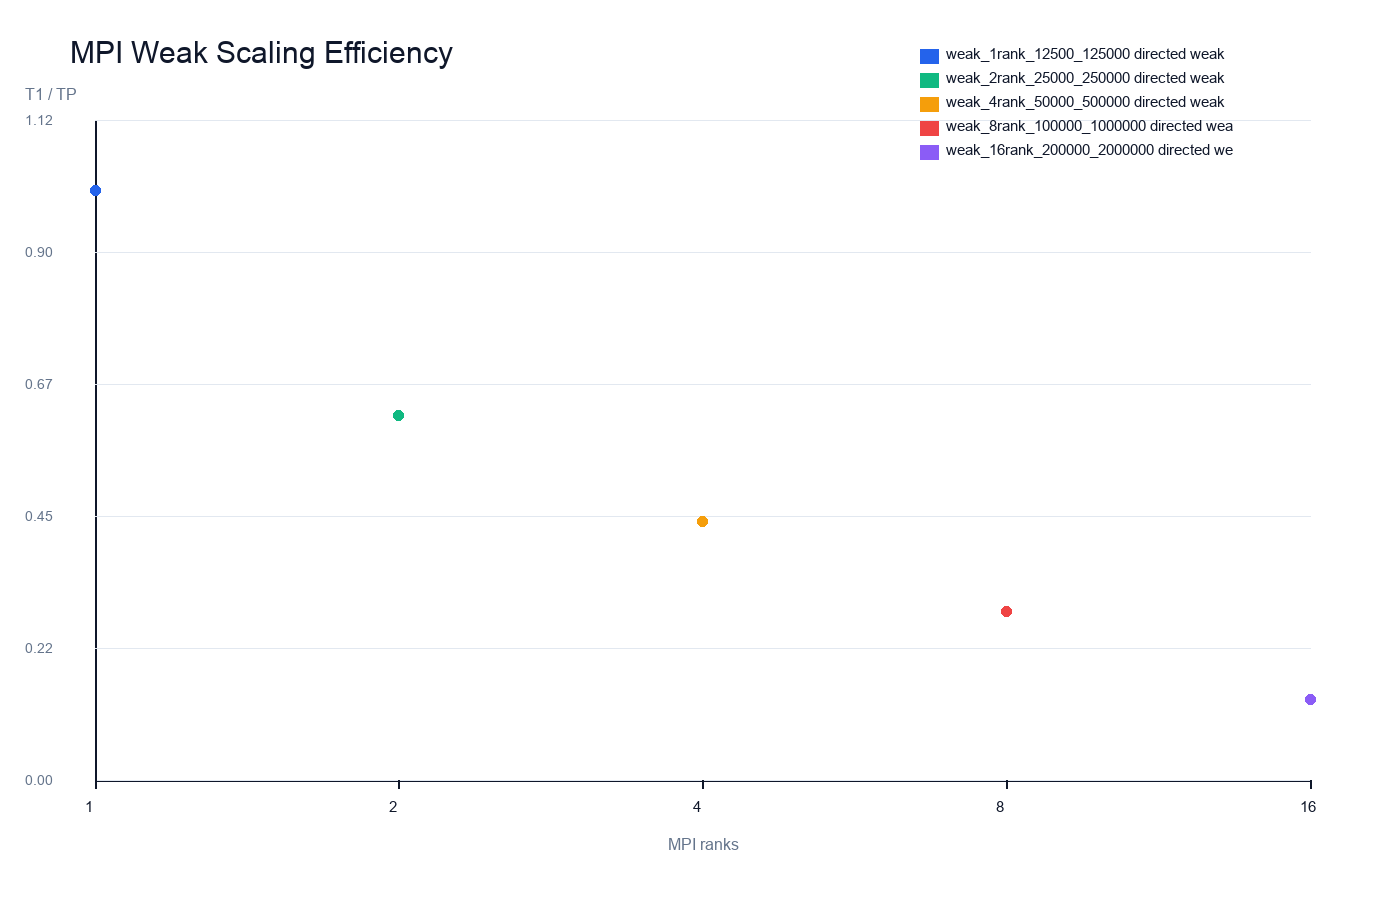
\includegraphics[width=0.48\textwidth]{results/figures/cluster_weak/mpi_weak_efficiency.png}
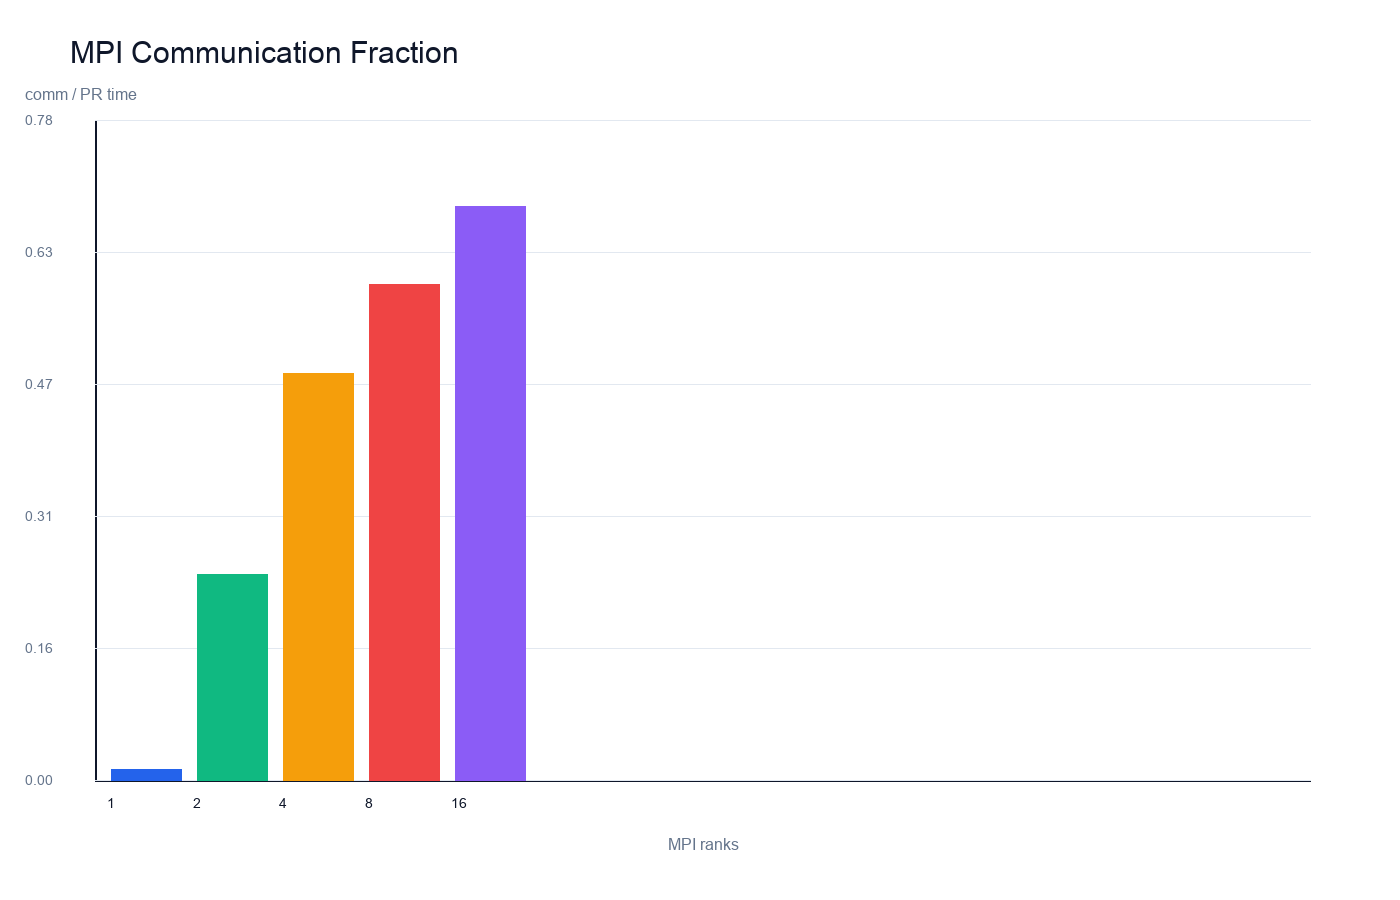
\includegraphics[width=0.48\textwidth]{results/figures/cluster_weak/mpi_comm_fraction.png}
\caption{School-cluster weak-scaling efficiency and communication fraction.}
\label{fig:wang-cluster-weak}
\end{figure}

\section{Optimization Effectiveness}
\label{sec:wang-optimization}

The first optimization is to precompute \texttt{inv\_out\_degree[u]} during
graph construction. The PageRank inner loop then uses multiplication instead of
performing a floating-point division for every incoming edge contribution:
\[
s_v = \sum_{u\in In(v)} pr_u \cdot \texttt{inv\_out\_degree[u]}.
\]
This directly targets the sparse-update kernel, which is the dominant
computation in the serial and single-rank paths.

The second optimization is the hybrid sparse-loop schedule. Because
destination vertices can have very different numbers of incoming edges,
\texttt{schedule(dynamic, 256)} reduces thread-level imbalance compared with a
pure static assignment. This does not remove MPI collective overhead, but it
improves the local work distribution within each rank for irregular graphs.

To verify these two choices directly, I added an ablation profiler that builds
four hybrid variants: \path{no_inv_static}, \path{inv_static},
\path{no_inv_dynamic}, and \path{inv_dynamic}. The intended comparison is run
at fixed total workers with \texttt{1x16} and \texttt{4x4}. The effectiveness
metrics are computed as
\[
\begin{aligned}
S_{\mathrm{inv}} &= T_{\mathrm{no\_inv\_static}} / T_{\mathrm{inv\_static}},\\
S_{\mathrm{dyn}} &= T_{\mathrm{inv\_static}} / T_{\mathrm{inv\_dynamic}}.
\end{aligned}
\]
and the full optimization speedup is
$T_{\mathrm{no\_inv\_static}}/T_{\mathrm{inv\_dynamic}}$. Table~\ref{tab:wang-optimization-ablation}
reports the measured school-cluster averages from the two
\path{results/optimization_ablation_cluster_*.csv} summary files; all variants
passed verification against the serial reference.

\begin{table}[H]
\centering
\caption{School-cluster optimization ablation, PR time in seconds.}
\label{tab:wang-optimization-ablation}
\scriptsize
\begin{tabular}{llrrrrr}
\toprule
Dataset & Config & No-inv static & Inv static & No-inv dyn. & Inv dyn. & Full speedup \\
\midrule
\texttt{synthetic\_100k\_1m} & \texttt{1x16} & 0.035235 & 0.033692 & 0.038780 & \textbf{0.030837} & \textbf{1.1426} \\
\texttt{synthetic\_100k\_1m} & \texttt{4x4}  & 0.012647 & 0.014116 & 0.012424 & \textbf{0.010092} & \textbf{1.2532} \\
\texttt{polblogs}            & \texttt{1x16} & 0.028250 & \textbf{0.023086} & 0.028299 & 0.026190 & 1.0787 \\
\texttt{polblogs}            & \texttt{4x4}  & \textbf{0.005697} & 0.008286 & 0.006149 & 0.005961 & 0.9557 \\
\bottomrule
\end{tabular}
\end{table}

The ablation results are mixed but useful. On the larger synthetic graph, the
fully optimized variant is best for both tested configurations: it improves
\texttt{1x16} by $1.1426\times$ and \texttt{4x4} by $1.2532\times$ over the
unoptimized static/division version. In the \texttt{4x4} case, dynamic
scheduling is the dominant local optimization, improving
\texttt{inv\_static} to \texttt{inv\_dynamic} by $1.3987\times$. On
\texttt{polblogs.csv}, the graph is small enough that timing noise and MPI
collective overhead hide some local kernel gains: precomputing
\texttt{inv\_out\_degree} helps the single-rank \texttt{1x16} case
($1.2237\times$), while the full \texttt{4x4} optimization is slightly slower
than the unoptimized baseline ($0.9557\times$).

OpenMP target execution was formally confirmed on the DD2356 Small GPU server:
the run detected one NVIDIA H100 \texttt{MIG 1g.10gb} target device, and
\texttt{omp\_is\_initial\_device()} confirmed that target regions executed on
device. On the directed \texttt{synthetic\_100k\_1m.csv} graph, retaining
arrays across PageRank iterations reduces average PR time from $0.059829$ s
for the naive path to $0.033684$ s for the persistent path, an improvement of
$1.7762\times$. Persistent offload is also slightly faster than the serial
reference for this kernel metric ($1.0822\times$). However, the same-server
Hybrid \texttt{4x2} control completes PR computation in $0.010364$ s, making
it $3.2500\times$ faster than persistent GPU offloading on this one-million-edge
input. Thus the data show a successful GPU optimization and a fair comparison,
but not a GPU win over the CPU hybrid implementation at the tested scale.

\begin{table}[H]
\centering
\caption{Confirmed-device GPU comparison on the DD2356 Small GPU server for
\texttt{synthetic\_100k\_1m.csv} (directed), five-run averages.}
\label{tab:wang-gpu-comparison}
\begin{tabular}{llll}
\toprule
Variant & Configuration & PR time (s) & Correctness \\
\midrule
Serial & 1 CPU thread & 0.036452 & reference \\
OpenMP target GPU & naive mapping & 0.059829 & PASS, device verified \\
OpenMP target GPU & persistent mapping & \textbf{0.033684} & PASS, device verified \\
Hybrid MPI+OpenMP & \texttt{4x2}, 8 CPU workers & \textbf{0.010364} & PASS \\
\bottomrule
\end{tabular}
\end{table}

\begin{figure}[H]
\centering
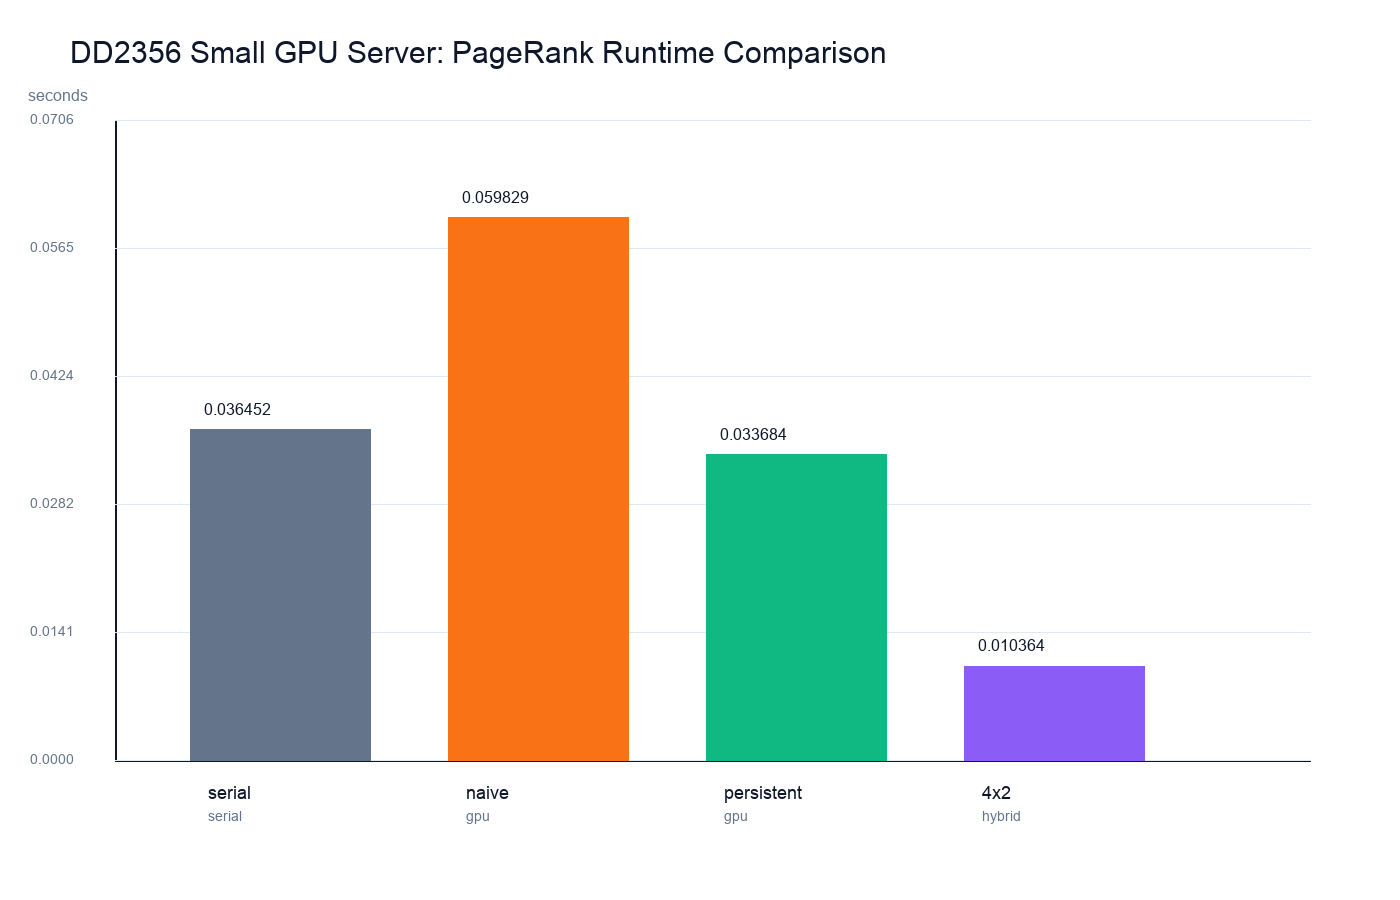
\includegraphics[width=0.48\textwidth]{results/figures/cluster_gpu/gpu_pr_time_comparison.png}
\hfill
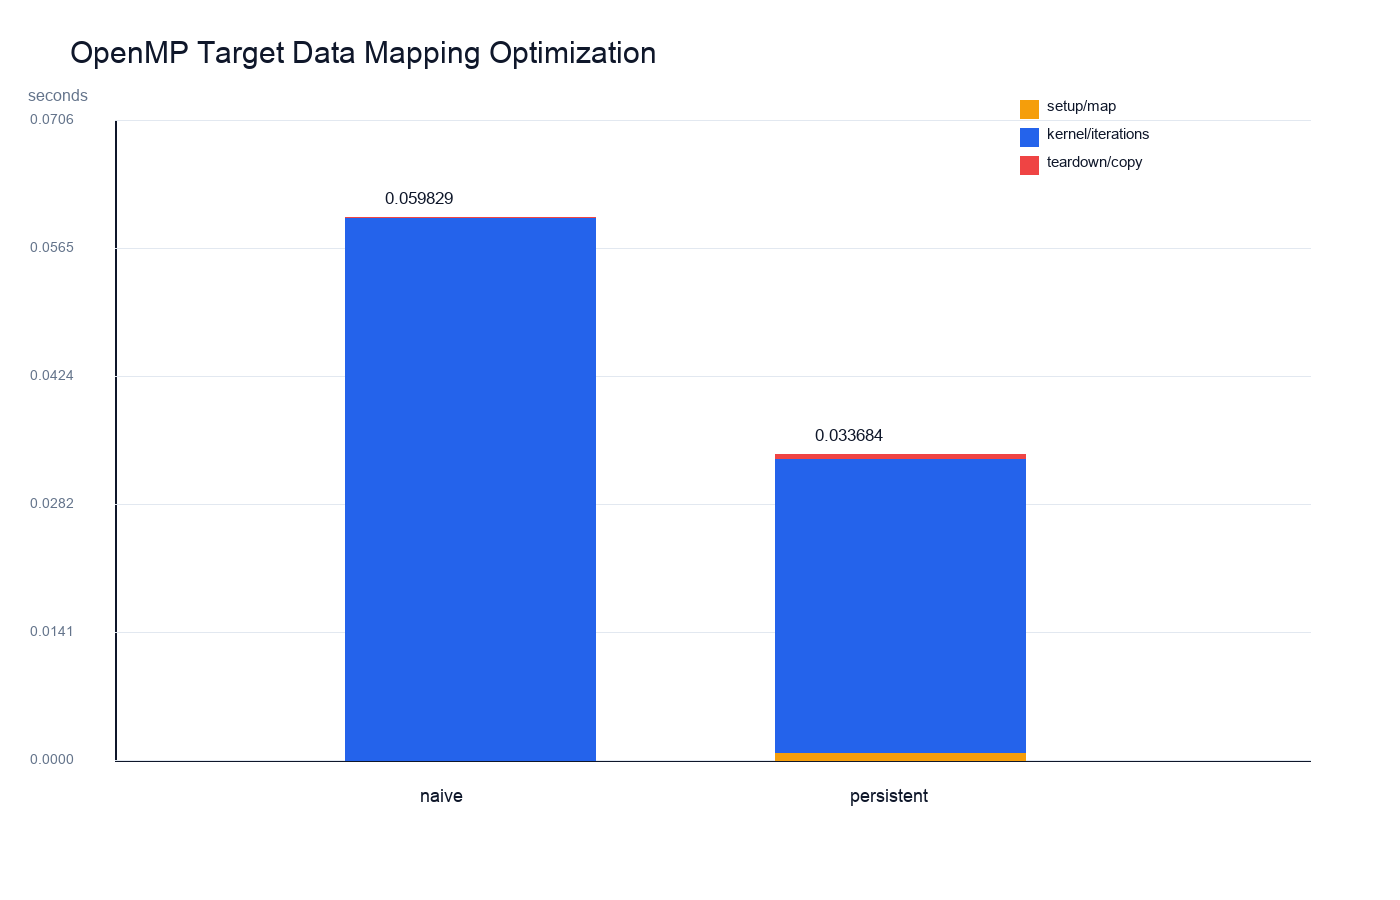
\includegraphics[width=0.48\textwidth]{results/figures/cluster_gpu/gpu_mapping_breakdown.png}
\caption{Same-server GPU and Hybrid timing comparison (left), and OpenMP
target mapping optimization breakdown (right).}
\label{fig:wang-gpu-comparison}
\end{figure}

For hybrid MPI+OpenMP, the fixed-core experiments keep the total number of CPU
workers at 16 and vary the split between MPI ranks and OpenMP threads. The
reported speedup is relative to the first fixed-core configuration
\texttt{1x16}; it is not a speedup over the serial baseline.

\begin{table}[H]
\centering
\caption{Hybrid fixed-core sweep on the school cluster for \texttt{polblogs.csv} (directed).}
\label{tab:wang-hybrid-polblogs}
\begin{tabular}{rrrrrr}
\toprule
Ranks & Threads/rank & PR time (s) & Comm frac. & Speedup vs. \texttt{1x16} & Status \\
\midrule
1  & 16 & 0.024310 & 0.0018 & 1.0000 & PASS \\
2  & 8  & 0.010850 & 0.1643 & 2.2406 & PASS \\
4  & 4  & 0.005325 & 0.7428 & 4.5652 & PASS \\
8  & 2  & 0.004281 & 0.8655 & 5.6783 & PASS \\
16 & 1  & \textbf{0.002907} & 0.9533 & \textbf{8.3631} & PASS \\
\bottomrule
\end{tabular}
\end{table}

\begin{table}[H]
\centering
\caption{Hybrid fixed-core sweep on the school cluster for \texttt{synthetic\_100k\_1m.csv} (directed).}
\label{tab:wang-hybrid-synth}
\begin{tabular}{rrrrrr}
\toprule
Ranks & Threads/rank & PR time (s) & Comm frac. & Speedup vs. \texttt{1x16} & Status \\
\midrule
1  & 16 & 0.036692 & 0.0137 & 1.0000 & PASS \\
2  & 8  & 0.018884 & 0.1758 & 1.9431 & PASS \\
4  & 4  & \textbf{0.011843} & 0.6741 & \textbf{3.0981} & PASS \\
8  & 2  & 0.019373 & 0.7682 & 1.8940 & PASS \\
16 & 1  & 0.012234 & 0.8220 & 2.9992 & PASS \\
\bottomrule
\end{tabular}
\end{table}

The best hybrid split depends on graph size. For \texttt{polblogs.csv}, the
best fixed-core result is \texttt{16x1}, which avoids OpenMP overhead and
benefits from the very small local work size despite high communication
fraction. For \texttt{synthetic\_100k\_1m.csv}, the best average result is
\texttt{4x4}: it exposes enough MPI parallelism while keeping collective
communication lower than the \texttt{8x2} and \texttt{16x1} configurations.

\section{A-Level Coverage and Remaining Measurements}
\label{sec:wang-coverage}

The Dardel \texttt{main}-partition job now closes the previously missing
multi-node MPI requirement: every multi-rank strong/weak row is placed across
\texttt{nid001120} and \texttt{nid001121}, and the 16-rank weak row uses the
required 200k-node/2M-edge graph. Confirmed-device OpenMP target measurements
on the DD2356 Small GPU server also close Wang's GPU-offloading comparison.
The remaining entries below belong to Minyi Zhu's OpenMP/hybrid analysis scope.

\begin{table}[H]
\centering
\caption{A-level evidence status after the current result consolidation.}
\label{tab:wang-remaining}
\small
\begin{tabular}{p{0.28\textwidth}p{0.31\textwidth}p{0.31\textwidth}}
\toprule
Requirement & Evidence available & Still required \\
\midrule
School-cluster MPI strong/weak scaling &
Strong and weak CSVs; weak includes verified 16-rank 200k/2M case &
Complete for measured rank sequence \\
Dardel MPI strong/weak scaling on multiple nodes &
Verified strong and weak CSVs for 1--16 ranks on two \texttt{main} nodes; hostname record &
Complete for measured rank sequence \\
Hybrid fixed-core search on school cluster &
Verified \texttt{1x16} through \texttt{16x1} sweeps &
Minyi scope: repeat for additional total core budgets \\
OpenMP speedup on three systems &
Correctness and local timing evidence &
Minyi scope: provide scaling measurements on three systems \\
GPU offload comparison with Hybrid &
Confirmed H100 MIG execution; nine-dataset PASS; same-server GPU naive/persistent and Hybrid \texttt{4x2} comparison &
Complete for Wang's GPU scope \\
\bottomrule
\end{tabular}
\end{table}

\section*{Contribution}
\label{sec:wang-contribution}

Pengyu Wang implemented the MPI decomposition and communication timing, ran and
analyzed the Dardel multi-node and school-cluster MPI strong/weak-scaling
experiments, added the 16-rank weak-scaling workflow with dynamically sized
graph readers, integrated the MPI result pipeline, and implemented and measured
OpenMP GPU offloading. The final GPU evidence confirms execution on an NVIDIA
H100 MIG device, demonstrates the persistent-device-data optimization against
the naive target baseline, and compares it with the group Hybrid
\texttt{4x2} baseline on the same server and graph.

\end{document}
